

\section{Assessments}

\section{Chapter 1, An Introduction to Inheritance and Polymorphism}

\begin{enumerate}
\item
  Objects and classes are the building blocks of a C++ program. By combining data and algorithms (\emph{code}) into a single unit, the C++ program represents the components of the system that it models, as well as their interactions.
\item
  Public inheritance represents an \emph{is-a} relationship between objects---an object of the derived class can be used as if it was an object of the base class. This relation implies that the interface of the base class, with its invariants and restrictions, is also a valid interface for the derived class.Unlike public inheritance, private inheritance says nothing about the interfaces. It expresses a \emph{has-a} or \emph{is implemented in terms of} relationship. The derived class reuses the implementation provided by the base class. For the most part, the same can be accomplished by composition. Composition should be preferred when possible; however, empty base optimization and (less often) virtual method overrides are valid reasons to use private inheritance.
\item
  A polymorphic object in C++ is an object whose behavior depends on its type, and the type is not known at compile time (at least at the point where the behavior in question is requested). An object that is referred to as a base class object can demonstrate the behavior of the derived class if that is its true type. In C++, polymorphic behavior is implemented using virtual functions.
\item
  Dynamic cast verifies at run time that the destination type of the cast is valid: it must be either the actual type of the object (the type the object was created with) or one if its base types. It is the latter part, checking all possible base types of an object, that makes dynamic casts expensive.
\end{enumerate}

\section{Chapter 2, Class and Function Templates}

\begin{enumerate}
\item
  A template is not a type; it is a \emph{Factory} for many different types with similar structures. A template is written in terms of generic types; substituting concrete types for these generic types results in a type generated from the template.
\item
  There are class, function, and variable templates. Each kind of template generates the corresponding entities---functions in the case of function templates, classes (types) from class templates, and variables from variable templates.
\item
  Templates can have type and non-type parameters. Type parameters are types. Non-type parameters can be integral or enumerated values or templates (in the case of variadic templates, the placeholders are also non-type parameters).
\item
  A template instantiation is the code generated by a template. Usually, the instantiations are implicit; the use of a template forces its instantiation. An explicit instantiation, without use, is also possible; it generates a type or a function that can be used later. An explicit specialization of a template is a specialization where all generic types are specified; it is not an instantiation, and no code is generated until the template is used. It is only an alternative recipe for generating code for these specific types.
\item
  Usually, the parameter pack is iterated over using recursion. The compiler will typically inline the code generated by this recursion, so the recursion exists only during compilation (as well as in the head of the programmer reading the code). In C++17 (and, rarely, in C++14), it is possible to operate on the entire pack without recursion.
\item
  Lambda expressions are essentially a compact way to declare local classes that can be called like functions. They are used to effectively store a fragment of code in a variable (or, rather, associate the code with a variable) so that this code can be called later.
\item
  Concepts impose restrictions on the template parameters. This can be used to avoid substituting types and instantiating a template that would lead to an error in the body of the template. In the more complex cases, concepts can be used to disambiguate the choice between multiple template overloads.
\end{enumerate}

\section{Chapter 3, Memory and Ownership}

\begin{enumerate}
\item
  Clear memory ownership, and by extension, resource ownership, is one of the key attributes of a good design. With clear ownership, resources are certain to be created and made available in time for when they are needed, maintained while they are in use, and released/cleaned up when no longer needed.
\item
  Resource leaks, including memory leaks; dangling handles (resource handles, such as pointers, references, or iterators, pointing to resources that do not exist); multiple attempts to release the same resource; multiple attempts to construct the same resource.
\item
  Non-ownership, exclusive ownership, shared ownership, as well as conversion between different types of ownership and transfer of ownership.
\item
  Ownership-agnostic functions and classes should refer to objects by raw pointers and references if the corresponding ownership is handled through owning pointers. If the objects are owned by rich pointers or containers, the problem becomes more difficult. If the additional data contained in the rich pointer is not needed or a single element of a container is accessed, raw pointers and references are perfectly adequate. Otherwise, ideally, we would use a corresponding non-owning reference object like \texttt{std::string\_view} or one of the views from the ranges library. If none is available, we may have to pass the owning object itself by reference.
\item
  Exclusive memory ownership is easier to understand and follow the control flow of the program. It is also more efficient.
\item
  Preferably, by allocating the object on the stack or as a data member of the owning class (including container classes). If reference semantics or certain move semantics are needed, a unique pointer should be used. For conditionally constructed objects, \texttt{std::optional} is a great solution.
\item
  Shared ownership should be expressed through a shared pointer such as \texttt{std::shared\_ptr}.
\item
  Shared ownership in a large system is difficult to manage and may delay the deallocation of resources unnecessarily. It also has a nontrivial performance overhead, compared to exclusive ownership. Maintaining shared ownership in a thread-safe concurrent program requires very careful implementation.
\item
  Views such as \texttt{std::string\_view}, \texttt{std::span}, and views from \texttt{std::ranges} are essentially non-owning rich pointers. A string view to a string is what a raw pointer is to a unique pointer: a non-owning object containing the same information as the corresponding owning object.
\end{enumerate}

\section{Chapter 4, Swap - From Simple to Subtle}

\begin{enumerate}
\item
  The swap function exchanges the state of the two objects. After the swap call, the objects should remain unchanged, except for the names they are accessed by.
\item
  Swap is usually employed in programs that provide commit-or-rollback semantics; a temporary copy of the result is created first, then swapped into its final destination only if no errors were detected.
\item
  The use of swap to provide commit-or-rollback semantics assumes that the swap operation itself cannot throw an exception or otherwise fail and leave the swapped objects in an undefined state.
\item
  A non-member swap function should always be provided, to ensure that the calls to non-member swap are executed correctly. A member swap function can also be provided, for two reasons---first, it is the only way to swap an object with a temporary, and second, the swap implementation usually needs access to the private data members of the class. If both are provided, the non-member function should call the member swap function on one of the two parameters.
\item
  All STL containers and some other standard library classes provide a member function \texttt{swap()}. In addition, the non-member \texttt{std::swap()\ }function template has standard overloads for all STL types.
\item
  The \texttt{std::\ qualifier} disables the argument-dependent lookup and forces the default \texttt{std::swap} template instantiation to be called, even if a custom swap function was implemented with the class. To avoid this problem, it is recommended to also provide an explicit instantiation of the \texttt{std::swap} template.
\end{enumerate}

\section{Chapter 5, Comprehensive Look at RAII}

\begin{enumerate}
\item
  Memory is the most common resource, but any object can be a resource. Any virtual or physical quantity that the program operates on is a resource.
\item
  Resources should not be lost (leaked). If a resource is accessed through a handle, such as a pointer or an ID, that handle should not be dangling (referring to a resource that does not exist). Resources should be released when they are no longer needed, in the manner that corresponds to the way they were acquired.
\item
  Resource Acquisition Is Initialization is an idiom; it is the dominant C++ approach to resource management, where each resource is owned by an object, acquired in the constructor, and released in the destructor of that object.
\item
  An RAII object should always be created on the stack or as a data member of another object. When the flow of the program leaves the scope containing the RAII object or the larger object containing the RAII object is deleted, the destructor of the RAII object is executed. This happens regardless of how the control flow leaves the scope.
\item
  If each resource is owned by an RAII object and the RAII object does not give out raw handles (or the user is careful to not clone the raw handle), the handle can only be obtained from the RAII object and the resource is not released as long as that object remains.
\item
  The most frequently used is \texttt{std::unique\_ptr} for memory management; \texttt{std::lock\_guard} is used to manage mutexes.
\item
  As a rule, RAII objects must be non-copyable. Moving an RAII object transfers the ownership of the resource; the classic RAII pattern does not support this, so most RAII objects should be non-movable (differentiate between \texttt{std::unique\_ptr} and \texttt{const\ std::unique\_ptr}).
\item
  RAII has difficulty handing release failures, because exceptions cannot propagate from the destructors, and hence there is no good way to report the failure to the caller. For that reason, failing to release a resource often results in undefined behavior (this approach is sometimes taken by the C++ standard as well).
\end{enumerate}

\section{Chapter 6, Understanding Type Erasure}

\begin{enumerate}
\item
  Type erasure is a programming technique where the program, as written, does not show an explicit dependence on some of the types it uses. It is a powerful design tool when used for separating abstract behavior from a particular implementation.
\item
  The implementation involves either a polymorphic object and a virtual function call, or a function that is implemented specifically for the erased type and is invoked through a function pointer. Usually, this is combined with generic programming to construct such polymorphic objects or generate functions from a template automatically and ensure that the reified type is always the same as the one provided during construction.
\item
  A program may be written in a way that avoids explicit mention of most types. The types are deduced by template functions and declared as \texttt{auto} or as template-deduced typedef types. However, the actual types of objects that are hidden by \texttt{auto} still depend on all types the object operates on (such as the deleter type for a pointer). The erased type is not captured by the object type at all. In other words, if you could get the compiler to tell you what this particular auto stands for, all types would be explicitly there. But if the type was erased, even the most detailed declaration of the containing object will not reveal it (such as \texttt{std::shared\_ptr\textless{}int\textgreater{}} ---this is the entire type, the deleter type is not there).
\item
  The type is reified by the function that is generated for that type: while its signature (arguments) does not depend on the erased type, the body of the function does. Usually, the first step is casting one of the arguments from a generic pointer such as \texttt{void*} to the pointer to the erased type.
\item
  The performance of type erasure always incurs some overhead compared to invoking the same callable directly: there is always an extra indirection and the pointer associated with it. Almost all implementations use runtime polymorphism (virtual functions or dynamic casts) or the equivalent virtual table of function pointers, which increases both the time (indirect function calls) and memory (virtual pointers). The greatest overhead usually comes from additional memory allocations, necessary for storing objects whose size is not known at compile time. If such allocations can be minimized and the additional memory made local to the object, the total overhead at runtime may be quite small (the overhead in memory remains and is often increased by such optimizations).
\end{enumerate}

\section{Chapter 7, SFINAE, Concepts, and Overload Resolution Management}

\begin{enumerate}
\item
  For each function call, it is the set of all functions with the specified name that are accessible from the call location (the accessibility may be affected by the namespaces, nested scopes, and so on).
\item
  It is the process of selecting which function in the overload set is going to be called, given the arguments and their types.
\item
  For template functions and member functions (and class constructors in C++17), type deduction determines the types of template parameters from the types of the function arguments. For each parameter, it may be possible to deduce the type from several arguments. In this case, the results of this deduction must be the same, otherwise, the type deduction fails. Once the template parameter types are deduced, the concrete types are substituted for the template parameters in all arguments, the return type, and the default arguments. This is a type substitution.
\item
  Type substitution, described previously, can result in invalid types, such as a member function pointer for a type that has no member functions. Such substitution failures do not generate compilation errors; instead, the failing overload is removed from the overload set.
\item
  This is only in the function declaration (return type, parameter types, and default values). Substitution failures in the body of the function chosen by the overload resolution are hard errors.
\item
  If each overload returns a different type, these types can be examined at compile time. The types must have some way to distinguish them, for example, different sizes or different values of embedded constants. For \texttt{constexpr} functions, we can also examine the return values (the function needs the body in this case).
\item
  It is used with great care and caution. By deliberately causing substitution failures, we can direct the overload resolution toward a particular overload. Generally, the desired overload is preferred unless it fails; otherwise, the variadic overload remains and is chosen, indicating that the expression we wanted to test was invalid. By differentiating between the overloads using their return types, we can generate a compile-time (\texttt{constexpr}) constant that can be used in conditional compilation.
\item
  C++20 constraints offer a more natural, easier-to-understand syntax. They also result in much clearer error messages when a called function does not meet the requirements. Also, unlike SFINAE, constraints are not limited to the substituted parameters of function templates.
\item
  The standard did not just define concepts and constraints in the language. It also offers a way of thinking about template restrictions. While a wide range of SFINAE-based techniques exists, the code is easier to read and maintain if the use of SFINAE is restricted to a few powerful approaches that resemble the use of concepts.
\end{enumerate}

\section{Chapter 8, The Curiously Recurring Template Pattern}

\begin{enumerate}
\item
  While not very expensive in absolute numbers (a few nanoseconds at most), a virtual function call is several times more expensive than a non-virtual one, and could easily be an order of magnitude or more slower than an inlined function call. The overhead comes from the indirection: a virtual function is always invoked by a function pointer, and the actual function is unknown at compile time and cannot be inlined.
\item
  If the compiler knows the exact function that is going to be called, it can optimize away the indirection and may be able to inline the function.
\item
  Just like the runtime polymorphic calls are made through the pointer to the base class, the static polymorphic calls must be also made through a pointer or reference to the base class. In the case of CRTP and static polymorphism, the base type is actually a whole collection of types generated by the base class template, one for each derived class. To make a polymorphic call we have to use a function template that can be instantiated on any of these base types.
\item
  When the derived class is called directly, the use of CRTP is quite different from the compile-time equivalent of the virtual functions. It becomes an implementation technique, where common functionality is provided to multiple derived classes, and each one expands and customizes the interface of the base class template.
\item
  Strictly speaking, nothing new is needed to use multiple CRTP bases: the derived class can inherit from several such base types, each an instantiation of a CRTP base class template. However, listing these based together with the correct template parameter (derived class itself) for each one becomes cumbersome. It is easier and less error-prone to declare the derived class as a variadic template with a template template parameter and inherit from the entire parameter pack.
\end{enumerate}

\section{Chapter 9, Named Arguments, Method Chaining, and the Builder Pattern}

\begin{enumerate}
\item
  It is easy to miscount arguments, change the wrong argument, or use an argument of the wrong type that happens to convert to the parameter type. Also, adding a new parameter requires changing all function signatures that must pass these parameters along.
\item
  The argument values within the aggregate have explicit names. Adding a new value does not require changing the function signatures. Classes made for different groups of arguments have different types and cannot be accidentally mixed.
\item
  The named argument idiom permits the use of temporary aggregate objects. Instead of changing each data member by name, we write a method to set the value of each argument. All such methods return a reference to the object itself and can be chained together in one statement.
\item
  Method cascading applies multiple methods to the same object. In a method chain, in general, each method returns a new object and the next method applies to it. Often, method chaining is used to cascade methods. In this case, all chained methods return the reference to the original object.
\item
  The Builder pattern is a design pattern that uses a separate builder object to construct complex objects. It is used when a constructor is not sufficient or not easy to use to construct an object in its desired fully built state. The need for a builder can arise when the constructor of the object being built cannot be modified (a general object used for a particular purpose), when a desired constructor would have many similar arguments and be hard to use when the construction process is complex, or when the construction process is computationally expensive but some of the results can be reused.
\item
  The fluent interface is an interface that uses method chaining to present multiple instructions, commands, or operations that can be executed on an object. In particular, fluent builders are used in C++ to split complex object construction into multiple smaller steps. Some of these steps can be conditional or depend on other data.
\end{enumerate}

\section{Chapter 10, Local Buffer Optimization}

\begin{enumerate}
\item
  Micro-benchmarks can measure the performance of small fragments of code in isolation. To measure the performance of the same fragment in the context of a program, we have to use a profiler.
\item
  Processing small amounts of data usually involve a correspondingly small amount of computing and are therefore very fast. Memory allocation adds a constant overhead, not proportional to the data size. The relative impact is larger when the processing time is short. In addition, memory allocation may use a global lock or otherwise serialize multiple threads.
\item
  Local buffer optimization replaces external memory allocation with a buffer that is a part of the object itself. This avoids the cost, and the overhead, of an additional memory allocation.
\item
  The object has to be constructed and the memory for it must be allocated, regardless of whether any secondary allocations happen. This allocation has some cost -- more if the object is allocated on the heap and less if it's a stack variable -- but that cost must be paid before the object can be used. Local buffer optimization increases the size of the object and therefore of the original allocation, but that usually does not significantly affect the cost of that allocation.
\item
  Short string optimization involves storing string characters in a local buffer contained inside the string object, up to a certain length of the string.
\item
  Small vector optimization involves storing a few elements of the vector's content in a local buffer contained in the vector object.
\end{enumerate}

\section{Chapter 11, ScopeGuard}

\begin{enumerate}
\item
  An error-safe program maintains a well-defined state (a set of invariants) even if it encounters an error. Exception safety is a particular kind of error safety; it assumes that errors are signaled by throwing expressions. The program must not enter an undefined state when an (allowed) expression is thrown. An exception-safe program may require that certain operations do not throw exceptions.
\item
  If a consistent state must be maintained across several actions, each of which may fail, then the prior actions must be undone if a subsequent action fails. This often requires that the actions do not commit fully until the end of the transaction is reached successfully. The final commit operation must not fail (for example, throw an exception), otherwise error safety cannot be guaranteed. The rollback operation also must not fail.
\item
  RAII classes ensure that a certain action is always taken when the program leaves a scope, such as a function. With RAII, the closing action cannot be skipped or bypassed, even if the function exits the scope prematurely with an early return or by throwing an exception.
\item
  The classic RAII needs a special class for every action. ScopeGuard automatically generates an RAII class from an arbitrary code fragment (at least, if lambda expressions are supported).
\item
  If the status is returned through error codes, it cannot. If all errors in the program are signaled by exceptions and any return from a function is a success, we can detect at runtime whether an exception was thrown. The complication is that the guarded operation may itself take place during stack unwinding caused by another exception. That exception is propagating when the guard class has to decide whether the operation succeeded or failed, but its presence does not indicate the failure of the guarded operation (it may indicate that something else failed elsewhere). Robust exception detection must keep track of how many exceptions are propagating at the beginning and at the end of the guarded scope, which is possible only in C++17 (or using compiler extensions).
\item
  The ScopeGuard classes are usually template instantiations. This means that the concrete type of the ScopeGuard is unknown to the programmer, or at least difficult to specify explicitly. The ScopeGuard relies on lifetime extension and template argument deduction to manage this complexity. A type-erased ScopeGuard is a concrete type; it does not depend on the code it holds. The downside is that type erasure requires runtime polymorphism and, most of the time, a memory allocation.
\end{enumerate}

\section{Chapter 12, Friend Factory}

\begin{enumerate}
\item
  A non-member friend function has the same access to the members of the class as a member function.
\item
  Granting friendship to a template makes every instantiation of this template a friend; this includes instantiations of the same template but with different, unrelated, types.
\item
  Binary operators implemented as member functions are always called on the left-hand-side operand of the operator, with no conversions allowed for that object. Conversions are allowed for the right-hand-side operand, according to the type of the argument of the member operator. This creates an asymmetry between expressions such as \texttt{x\ +\ 2} and \texttt{2\ +\ x}, where the latter cannot be handled by a member function since the type of \texttt{2} (\texttt{int}) does not have any.
\item
  The first operand of the inserter is always the stream, not the object that is printed. Therefore, a member function would have to be on that stream, which is a part of the standard library; it cannot be extended by the user to include user-defined types.
\item
  While the details are complex, the main difference is that user-defined conversions (implicit constructors and conversion operators) are considered when calling non-template functions but, for template functions, the argument types must match the parameter types (almost) exactly, and no user-defined conversions are permitted.
\item
  Defining an in situ friend function (with the definition immediately following the declaration) in a class template causes every instantiation of that template to generate one non-template, non-member function with the given name and parameter types in the containing scope.
\end{enumerate}

\section{Chapter 13, Virtual Constructors and Factories}

\begin{enumerate}
\item
  There are several reasons, but the simplest is that the memory must be allocated in the amount \texttt{sizeof(T)}, where \texttt{T} is the actual object type, and the \texttt{sizeof()} operator is \texttt{constexpr} (a compile-time constant).
\item
  The Factory pattern is a creational pattern that solves the problem of creating objects without having to explicitly specify the type of the object.
\item
  While in C++ the actual type has to be specified at the construction point, the Factory pattern allows us to separate the point of construction from the place where the program has to decide what object to construct and identify the type using some alternative identifier, a number, a value, or another type.
\item
  The virtual copy constructor is a particular kind of factory where the object to construct is identified by the type of another object we already have. A typical implementation involves a virtual \texttt{clone()} method that is overridden in every derived class.
\item
  The Template pattern describes the design where the overall control flow is dictated by the base class, with derived classes providing customizations at certain predefined points. In our case, the overall control flow is that of factory construction, and the customization point is the act of construction of an object (memory allocation and constructor invocation).
\item
  The Builder pattern is used when it is necessary (or just more convenient) to delegate the work of constructing an object to another class instead of doing the complete initialization in the constructor. An object that constructs other objects of different types depending on some run-time information using the factory method is also a builder. In addition to the factory itself, such builders, or factory classes, usually have other run-time data that is used for constructing objects and must be stored in another object -- in our case, the factory object, which is also the builder object.
\end{enumerate}

\section{Chapter 14, The Template Method Pattern and the Non-Virtual Idiom}

\begin{enumerate}
\item
  A behavioral pattern describes a way to solve a common problem by using a specific method to communicate between different objects.
\item
  The template method pattern is a standard way to implement an algorithm that has a rigid \emph{skeleton,} or the overall flow of control, but allows for one or more customization points for specific kinds of problems.
\item
  The Template Method lets the sub-classes (derived types) implement specific behaviors of the otherwise generic algorithm. The key to this pattern is the way the base and the derived types interact.
\item
  The more common hierarchical approach to design sees the low-level code provide \emph{building blocks} from which the high-level code builds the specific algorithm, by combining them in a particular flow of control. In the template pattern, the high-level code does not determine the overall algorithm and is not in control of the overall flow. The lower-level code controls the algorithm and determines when the high-level code is called to adjust specific aspects of the execution.
\item
  It is a pattern where the public interface of a class hierarchy is implemented by non-virtual public methods of the base class and the derived classes contain only virtual private methods (as well as any necessary data and non-virtual methods needed to implement them).
\item
  A public virtual function performs two separate tasks -- it provides the interface (since it is public) and also modifies the implementation. A better separation of concerns is to use virtual functions only to customize the implementation and to specify the common interface using the non-virtual functions of the base class.
\item
  Once the NVI is employed, virtual functions can usually be made private. One exception is when the derived class needs to invoke a virtual function of the base class to delegate part of the implementation. In this case, the function should be made protected.
\item
  Destructors are called in \emph{nested} order, starting from the most derived class. When the destructor for the derived class is done, it calls the destructor of the base class. By that time, the \emph{extra} information that the derived class contained is already destroyed, and only the base portion is left. If the base class destructor were to call a virtual function, it would have to be dispatched to the base class (since the derived class is gone by then). There is no way for the base class destructor to call the virtual functions of the derived class.
\item
  The fragile base class problem manifests itself when a change to the base class unintentionally breaks the derived class. While not specific to the template method, it affects, potentially, all object-oriented designs, including ones based on the template pattern. In the simplest example, changing the non-virtual public function in the base class, in a way that changes the names of the virtual functions called to customize the behavior of the algorithm, will break all existing derived classes because their current customizations, implemented by the virtual functions with the old names, would suddenly stop working. To avoid this problem, the existing customization points should not be changed.
\end{enumerate}

\section{Chapter 15, Policy-Based Design}

\begin{enumerate}
\item
  The Strategy pattern is a behavioral pattern that allows the user to customize a certain aspect of the behavior of the class by selecting an algorithm that implements this behavior from a set of provided alternatives, or by providing a new implementation.
\item
  While the traditional OOP Strategy applies at runtime, C++ combines generic programming with the Strategy pattern in a technique known as policy-based design. In this approach, the primary class template delegates certain aspects of its behavior to the user-specified policy types.
\item
  In general, there are almost no restrictions on the policy type, although the particular way in which the type is declared and used imposes certain restrictions by convention. For example, if a policy is invoked as a function, then any callable type can be used. On the other hand, if a specific member function of the policy is called, the policy must necessarily be a class and provide the required member function. Template policies can be used as well but must match the specified number of template parameters exactly.
\item
  The two primary ways are composition and inheritance. The composition should generally be preferred; however, many policies in practice are empty classes with no data members and can benefit from empty base class optimization. Private inheritance should be preferred unless the policy must also modify the public interface of the primary class. Policies that need to operate on the primary policy-based class itself often have to employ CRTP. In other cases, when the policy object itself does not depend on the types used in the construction of the primary template, the policy behavior can be exposed through a static member function.
\item
  As a general rule, policies that contain only constants and are used to constrain the public interface are easier to write and maintain. However, there are several cases when injecting public member functions through the base class policies is preferred: when we also need to add member variables to the class or when the complete set of public functions would be difficult to maintain or lead to conflicts.
\item
  The primary drawback is complexity, in various manifestations. Policy-based types with different policies are, generally, different types (the only alternative, type erasure, usually carries a prohibitive runtime overhead). This may force large parts of the code to be templated as well. Long lists of policies are difficult to maintain and use correctly. For this reason, care should be taken to avoid creating unnecessary or hard-to-justify policies. Sometimes a type with two sufficiently unrelated sets of policies is better to be split into two separate types.
\end{enumerate}

\section{Chapter 16, Adapters and Decorators}

\begin{enumerate}
\item
  The Adapter is a very general pattern that modifies an interface of a class or a function (or a template, in C++) so it can be used in a context that requires a different interface but similar underlying behavior.
\item
  The Decorator pattern is a more narrow pattern; it modifies the existing interface by adding or removing behavior but does not convert an interface into a completely different one.
\item
  In the classic OOP implementation, both the decorated class and the Decorator class inherit from a common base class. This has two limitations; the most important one is that the decorated object preserves the polymorphic behavior of the decorated class but cannot preserve the interface that is added in a concrete (derived) decorated class and was not present in the base class. The second limitation is that the Decorator is specific to a particular hierarchy. We can remove both limitations using the generic programming tools of C++.
\item
  In general, a Decorator preserves as much of the interface of the decorated class as possible. Any functions the behavior of which is not modified are left unchanged. For that reason, public inheritance is commonly used. If a Decorator has to forward most calls to the decorated class explicitly, then the inheritance aspect is less important, and composition or private inheritance can be used.
\item
  Unlike Decorators, adapters usually present a very different interface from that of the original class. Composition is often preferred in this case. The exception is compile-time adapters that modify the template parameters but otherwise are essentially the same class template (similar to template aliases). These adapters must use public inheritance.
\item
  The main limitation is that it cannot be applied to template functions. It also cannot be used to replace function arguments with expressions containing those arguments.
\item
  Template aliases are never considered by the argument type deduction when function templates are instantiated. Both adapter and policy patterns can be used to add or modify the public interface of a class.
\item
  Adapters are easy to stack (compose) to build a complex interface one function at a time. The features that are not enabled do not need any special treatment at all; if the corresponding adapter is not used, then that feature is not enabled. The traditional policy pattern requires predetermined slots for every pattern. With the exception of the default arguments after the last explicitly specified one, all policies, even the default ones, must be explicitly specified. On the other hand, the adapters in the middle of the stack do not have access to the final type of the object, which complicates the implementation. The policy-based class is always the final type, and using CRTP, this type can be propagated into the policies that need it.
\end{enumerate}

\section{Chapter 17, The Visitor Pattern and Multiple Dispatch}

\begin{enumerate}
\item
  The Visitor pattern provides a way to separate the implementation of algorithms from the objects they operate on; in other words, it is a way to add operations to classes without modifying them by writing new member functions.
\item
  The Visitor pattern allows us to extend the functionality of class hierarchies. It can be used when the source code of the class is not available for modification or when such modifications would be difficult to maintain.
\item
  Double dispatch is the process of dispatching a function call (selecting the algorithm to run) based on two factors. Double dispatch can be implemented at runtime using the Visitor pattern (virtual functions provide the single dispatch) or at compile time using templates or compile-time visitors.
\item
  The classic visitor has a circular dependency between the visitor class hierarchy and the visitable class hierarchy. While the visitable classes do not need to be edited when a new visitor is added, they do need to be recompiled when the visitor hierarchy changes. The latter must happen every time a new visitable class is added, hence a dependency circle. The Acyclic Visitor breaks this circle by using cross-casting and multiple inheritance.
\item
  A natural way to accept a visitor into an object composed of smaller objects is to visit each of these objects one by one. This pattern, implemented recursively, ends up visiting every built-in data member contained in an object and does so in a fixed, predetermined order. Hence, the pattern maps naturally onto the requirement for serialization and deserialization, where we must deconstruct an object into a collection of built-in types, then restore it.
\end{enumerate}

\section{Chapter 18, Patterns for Concurrency}

\begin{enumerate}
\item
  Concurrency is the property of a program that allows multiple tasks to execute at the same time or partially overlapping in time. Usually, concurrency is achieved through the use of multiple threads.
\item
  C++11 has the basic support for writing concurrent programs: threads, mutexes, and condition variables. C++14 and C++17 added several convenience classes and utilities, but the next major addition to concurrency features of C++ is C++20: here, we have several new synchronization primitives as well as the introduction of the coroutines.
\item
  Synchronization patterns are the common solutions to the basic problems of accessing shared data. Usually, they provide ways to arrange exclusive access to the data that is modified by multiple threads or is accessed by some threads while being modified by others.
\item
  Execution patterns are the standard ways to arrange asynchronous execution of some computations using one or more threads. These patterns offer ways to initiate the execution of some code and receive the results of this execution without the caller being responsible for the execution itself (some other entity in the program has that duty).
\item
  The most important guideline for design for concurrency is modularity; when applies specifically to concurrency, it means building concurrent software from components that satisfy certain restrictions on their behavior in concurrent programs. The most important of these restrictions is the thread safety guarantee: generally, it is much easier to build concurrent software from components that allow a wide range of thread-safe operations.
\item
  In order to be useful in concurrent programs, any data structure or component must provide a transactional interface. An operation is a transaction if it performs a well-defined complete computation and leaves the system in a well-defined state. A simplified way to identify which operations are and are not transactions is this: if a concurrent program executes each operation under lock but there are no order guarantees between the operations, is the state of the system guaranteed to be well-defined? If it isn't, then some of the operations should be executed as a sequence without releasing the lock. That sequence is a transaction; the operations that are the steps of the sequence are not transactions by themselves. It should not be the responsibility of the caller to arrange these operations in a sequence. Instead, the data structure or component should offer the interface for performing the entire transaction as a single operation.
\end{enumerate}


\section{Index}

As this ebook edition doesn\textquotesingle t have fixed pagination, the page numbers below are hyperlinked for reference only, based on the printed edition of this book.

A

abstract class 13

Active Object 565-569

Acyclic Visitor pattern 509-512

Adapter pattern 455-459

compile-time adapters 464-469

function adapters 459-462

versus Decorator pattern 462-464

Adapter solution 470-479

versus policy solution 469, 470

address sanitizer (ASAN) 399

advanced policy-based design 410

adapters and aliases 420-422

policies, for constructors 410-417

policies, for test 417-420

policies, rebinding 431, 432

policies, using to control public interface 422-430

aggregate parameters 230, 231

argument-dependent lookup (ADL) 90, 325

arguments

problem 226-229

B

Barton-Nackman trick 331

Builder pattern 242

basics 243, 244

fluent builder 244-250

implicit builder 250-254

C

C++ 538

coroutine patterns 574-577

friends 317

friendship, granting in 317, 318

function overloading 157-159

NVI idiom 376-378

resource management 96

template functions 159, 161

Template Method pattern 369

type erasure, implementing 135

Visitor pattern 492-496

C++11 82

C++17 82

Visitor pattern 530-535

C++20

concepts 175-177

constraints 172-175

SFINAE techniques 177, 179

type restrictions 176, 177

C++, named arguments 232

method chaining 232

C++ template machinery

concepts 52-56

cascading-by-chaining by returning self 239

char argument 53

circular buffer 270, 562

classes 4, 5

class hierarchies 5-11

method chaining 239-242

class templates 23

instantiations 31-34

class wrappers 455

compile-time adapters 464-469

compile-time polymorphism 205, 206

compile-time pure virtual function 206-208

complex objects

visiting 500

composite objects

visiting 500-502

composition 9, 403

concurrency 538

concurrent design

patterns and guidelines 556

concurrent design, patterns and guidelines

data structures, with access limitations 561-564

thread safety guarantees 556, 557

transactional interface design 557-561

concurrent execution patterns 564

active object 565-569

Monitor pattern 571-573

Proactor Object pattern 570, 571

Reactor Object pattern 569, 570

condition pattern 547

constructor template argument deduction (CTAD) 395

copy-and-swap 86

copy elision 70

Copy On Write (COW) 284

coroutine patterns

in C++ 574-577

covariant return types 12

cross-cast 17

CRTP, as delegation pattern 211

concepts, using with 214-216

interface, expanding 212, 213

CRTP, as implementation technique 216

for code reuse 216-218

for generic interfaces 218-220

Curiously Recurring Template Pattern (CRTP) 197-204, 333-335, 359, 406, 444, 513

access control 210, 211

as delegation pattern 211

as implementation technique 216

policy-based design 221-223

static polymorphism 205

D

declarative programming 294

Decorator pattern 440-444

C++ way 444-449

composable decorators 453-455

versus Adapter pattern 462-464

destructors 380-382

double dispatch 490

E

empty base class optimization 404

encapsulation 4

error handling 288

error safety 288-291

exception safety 288-291

explicit template specialization 34, 36

F

factory-like patterns, C++ 357

CRTP Factory 358-360

CRTP, for Factory implementation 360, 361

Factory and Builder 361-364

polymorphic copy 357, 358

return types 358-360

factory method

arguments 346-350

basics 342-344

factory pattern 342

clarification 344-346

dynamic type registry 350-355

polymorphic factory 355, 357

fluent builder 244-250

Fragile Base Class problem 383, 384

friend factory pattern 333-335

friends, C++ 317

and templates 328

subtle details 322-327

versus member function 318-322

function adapters 459-462

function overloading 157-159

function template 22, 23

instantiations 28-31

functors 47

G

Generic Acyclic Visitor 519-523

Generic Visitor 512-515

H

handle-body idiom 89

I

imperative programming 294

implicit builder 250-254

inaccessible base 15

inheritance 5-11

K

Koenig lookup 90, 325

L

lambda expression 47-52

Lambda Visitor 515-519

local buffer optimization 261

additional optimizations 267

effects 264-266

example 261-264

limitations 284

overview 276-284

local buffer optimization, strings 267

callable objects 272-275

in standard library 275

small queue 270, 271

small vector 268-270

type-erased 272-275

lock-free synchronization patterns 551-556

M

manual resource management

disadvantages 101

manual resource management, disadvantages

error-prone 101-104

exception safety 104, 105

member functions

versus friends 318-322

memory barriers 549

memory management 96

memory ownership 60-62

exclusive ownership 64, 65

non-ownership 63, 64

poorly designed memory ownership 61, 62

shared ownership 67, 68

transfer of exclusive ownership 65, 66

well-designed memory ownership 60, 61

method cascading 238

versus method chaining 238, 239

method chaining 232-239

in class hierarchies 239-242

versus method cascading 238, 239

micro-benchmark library

installing 148

modern C++

Visitor pattern 512

Monitor pattern 571-573

moved-from 91

move elision 70

multiple inheritance 17-19

mutual exclusion (mutex) 539

MySwap() function 55

N

named arguments 233, 234

in C++ 232

performance 235-237

non-member swap 82

non-type template parameters 24-26

Non-Virtual Interface (NVI)

access 375, 376

destructors 380-382

Template Method pattern, versus Strategy pattern 379

virtual functions 375, 376

Non-Virtual Interface (NVI), drawbacks

composability 382, 383

Fragile Base Class problem 383, 384

template customization points 384-386

NVI idiom

in C++ 376-378

O

object ownership 60

objects 3-5

owning 69

type, obtaining 338-342

OO programming (OOP) 3-5

open/closed principle 490

operator\textless() method 53

overload set 159

P

partial template specializations 36-39

pimpl idiom 89

policy-based design 221, 392

disadvantages 434, 435

foundations of 392-399

guidelines 435, 437

policies, implementing 400-403

policy objects, using 403-410

strengths 433

policy solution 479-486

versus Adapter policy 469, 470

polymorphic 12

polymorphic decorators 449-453

limitations 449-453

polymorphism 11-17

polymorphism, CRTP 205

compile-time polymorphism 205, 206

compile-time pure virtual function 206-208

destructors 208, 209

polymorphic deletion 208, 209

private inheritance 9

Proactor Object pattern 570, 571

pure virtual 13

R

RAII idiom 288-294

Reactor Object pattern 569, 570

reification 136

requires expression 54

requires keyword 53

Resource Acquisition is Initialization (RAII) 95, 106-111, 393

downsides 118-120

for other resources 111, 112

modern techniques 120-124

objects, implementation 116-118

resources, releasing 112-115

resource management, C++ 96

Google Test, installing 98

microbenchmark library, installing 96-98

resources, counting 99, 100

resource ownership 60

resource-owning objects 69-71

non-owning access to 71-75

ring buffer 270

runtime 210

runtime polymorphism 12

Run-Time Type Information (RTTI) 217

S

ScopeGuard exception 305

commit() function, executing 308-312

commit() function, throwing 306-308

ScopeGuard pattern 295

basics 295-300

generic version 300-305

serialization, and deserialization

issues, solving with Visitor pattern 502-509

several base classes

multiple inheritance 17-19

SFINAE, constrained templates

best practices 191, 192

SFINAE techniques

concepts, before concepts 183-191

in C++20 177-179

type traits 179-183

shielded ScopeGuard 307

short string optimization 263

single dispatch 491

small memory allocations 258

cost measures 258-261

Smalltalk 232

Standard Template Library (STL) 525

Standard Template Library (STL), containers 80-82

swap, handling 83

static interface 211

Strategy pattern 392

versus Template Method pattern 379

Substitution 425

Substitution Failure Is Not An Error (SFINAE) 165-167

techniques 177

swap

exception safety 84-86

handling, in STL containers 83

idioms 86, 87

implementing 88-91

implementing and using, correctly 88

need for 83

using, correctly 91-93

swap() function 55

swap operation 80-82

synchronization patterns 538

data sharing, approaches 542-547

lock-free synchronization patterns 551-556

locking patterns 539-542

mutex pattern 539-542

waiting 547-551

T

template classes

friends 328-330

template customization points 384-386

template friend factory 331

friends on demand, generating 331-333

template functions 159-161

overloading 39-42

type substitution 161

template instantiations 28

Template Method pattern 367, 368

actions 371-374

applications of 369-371

in C++ 369

pre-and post-conditions 371-374

versus Strategy pattern 379

templates, in C++ 21

class templates 23

function templates 22, 23

non-type template parameters 24-26

template template parameters 26, 27

variable templates 24

template template parameters 26, 27

test fixture 100

thread safety guarantees 556

levels 556

thread sanitizer (TSAN) 540

transactional interface design 557-561

type deduction 162, 163

type-erased ScopeGuard 312-315

type erasure 127, 128

as design pattern 133

as implementation technique 134, 135

example 128-131

example to generalization 132

using, guidelines 152, 153

type erasure, in C++

efficiency 144-148

implementing 135

inheritance, using 137

predates 136, 137

without inheritance 139-143

without memory allocation 138, 139

type erasure, performance

micro-benchmark library, installing 148

overhead 148-152

typename keyword 55

type substitution 162, 163

failure 163-165

failure, encountering 169-172

failure, error 167, 168

in template functions 161

type traits 179-183

V

variable templates 24

variadic templates 42-46

views

owning 69

virtual functions 11-17

limitations 198-200

Visitor pattern 490-492

complex objects, visiting 500

composite objects, visiting 500-502

deserialization with 502-509

generalizations and limitations 496-500

in C++ 492-496

in C++17 530-535

in modern C++ 512

serialization with 502-509

using, at compile time 523-530

Visitor pattern, in modern C++

Acyclic Visitor pattern 519-523

Generic Visitor 512-515

Lambda Visitor 515-519

v-pointer 337


\pandocbounded{
\includegraphics[keepaspectratio]{./image/Packt_Logo_SuperSite_2022_Orange1.png}}

www.packtpub.com

Subscribe to our online digital library for full access to over 7,000 books and videos, as well as industry leading tools to help you plan your personal development and advance your career. For more information, please visit our website.

\section{Why subscribe?}

\begin{itemize}
\item
  Spend less time learning and more time coding with practical eBooks and Videos from over 4,000 industry professionals
\item
  Improve your learning with Skill Plans built especially for you
\item
  Get a free eBook or video every month
\item
  Fully searchable for easy access to vital information
\item
  Copy and paste, print, and bookmark content
\end{itemize}

Did you know that Packt offers eBook versions of every book published, with PDF and ePub files available? You can upgrade to the eBook version at packtpub.com and as a print book customer, you are entitled to a discount on the eBook copy. Get in touch with us at customercare@packtpub.com for more details.

At www.packtpub.com, you can also read a collection of free technical articles, sign up for a range of free newsletters, and receive exclusive discounts and offers on Packt books and eBooks.

\section{Other Books You May Enjoy}

If you enjoyed this book, you may be interested in these other books by Packt:

\pandocbounded{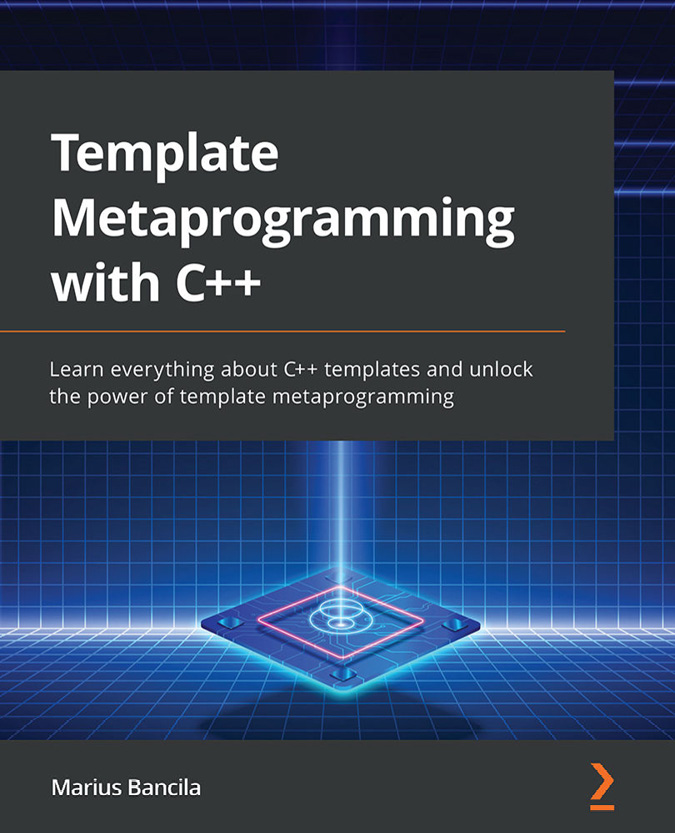
\includegraphics[keepaspectratio]{./image/9781803243450_Cover.jpg}}

\textbf{Template Metaprogramming} \textbf{with C++}

Marius Bancila

ISBN: 978-1-80324-345-0

\begin{itemize}
\item
  Understand the syntax for all types of templates
\item
  Discover how specialization and instantiation works
\item
  Get to grips with template argument deduction and forwarding references
\item
  Write variadic templates with ease
\item
  Become familiar with type traits and conditional compilation
\item
  Restrict template arguments in C++20 with constraints and concepts
\item
  Implement patterns such as CRTP, mixins, and tag dispatching
\end{itemize}

\pandocbounded{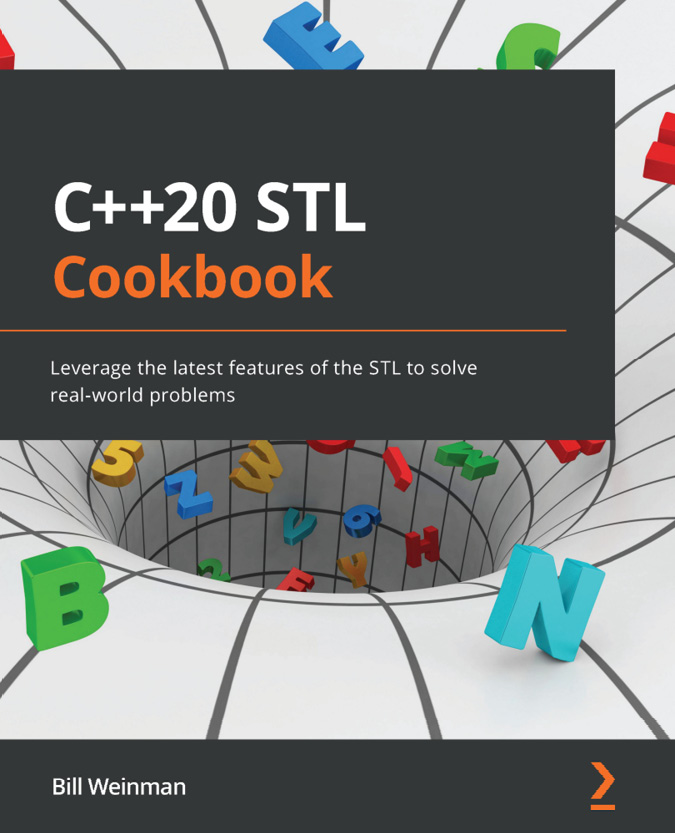
\includegraphics[keepaspectratio]{./image/9781803248714_Cover.jpg}}

\textbf{C++20} \textbf{STL Cookbook}

Bill Weinman

ISBN: 978-1-80324-871-4

\begin{itemize}
\item
  Understand the new language features and the problems they can solve
\item
  Implement generic features of the STL with practical examples
\item
  Understand standard support classes for concurrency and synchronization
\item
  Perform efficient memory management using the STL
\item
  Implement seamless formatting using std::format
\item
  Work with strings the STL way instead of handcrafting C-style code
\end{itemize}

\section{Packt is searching for authors like you}

If you're interested in becoming an author for Packt, please visit authors.packtpub.com and apply today. We have worked with thousands of developers and tech professionals, just like you, to help them share their insight with the global tech community. You can make a general application, apply for a specific hot topic that we are recruiting an author for, or submit your own idea.

\section{Share your thoughts}

Now you've finished \emph{Hands-On Design Patterns with C++ (Second Edition)}, we'd love to hear your thoughts! If you purchased the book from Amazon, please click here to go straight to the Amazon review page for this book and share your feedback or leave a review on the site that you purchased it from.

Your review is important to us and the tech community and will help us make sure we're delivering excellent quality content.

\section{Download a free PDF copy of this book}

Thanks for purchasing this book!

Do you like to read on the go but are unable to carry your print books everywhere?

Is your eBook purchase not compatible with the device of your choice?

Don't worry, now with every Packt book you get a DRM-free PDF version of that book at no cost.

Read anywhere, any place, on any device. Search, copy, and paste code from your favorite technical books directly into your application.

The perks don't stop there, you can get exclusive access to discounts, newsletters, and great free content in your inbox daily

Follow these simple steps to get the benefits:

\begin{enumerate}
\item
  Scan the QR code or visit the link below
\end{enumerate}

\pandocbounded{
\includegraphics[keepaspectratio]{./image/B19262_QR_Free_PDF.jpg}}

https://packt.link/free-ebook/9781804611555

\begin{enumerate}
\item
  Submit your proof of purchase
\item
  That's it! We'll send your free PDF and other benefits to your email directly
\end{enumerate}
